\documentclass{article}
\usepackage[utf8]{inputenc}
\usepackage{graphicx}
\usepackage[fleqn, leqno]{mathtools} 
\usepackage{textcomp}
\usepackage{titling}
\usepackage{subfig}
\usepackage[parfill]{parskip}
\usepackage{xcolor}
\definecolor{LightGray}{gray}{0.9}
\usepackage{titlesec}
\setcounter{secnumdepth}{4}
\usepackage[a4paper,left=1cm,right=1cm,top=1cm,bottom=1.5cm,]{geometry}
\usepackage{eqparbox}
\usepackage{enumitem}
\usepackage{relsize}
\usepackage{dsfont}

\newcommand*{\vertbar}{\rule[-1ex]{0.5pt}{2.5ex}}
\newcommand*{\horzbar}{\rule[.5ex]{2.5ex}{0.5pt}}

\makeatletter
\newcommand{\leqnomode}{\tagsleft@true\let\veqno\@@leqno}
\newcommand{\reqnomode}{\tagsleft@false\let\veqno\@@eqno}
\makeatother

\counterwithin*{equation}{section}
\counterwithin*{equation}{subsection}
\counterwithin*{equation}{subsubsection}

\title{\vspace{-2cm} CS231N Assignment 1 - Matrix Calculus, 2-layer NN}
\date{\vspace{-5ex}}

\begin{document}
\maketitle

\section{Matrix Calculus}

\subsection{Derivative of Vector wrt Matrix}
\begin{subequations}
    \renewcommand{\theequation}{\theparentequation.\arabic{equation}}
    \begin{equation}
        \text{We have vector } \boldsymbol{r} = \begin{bmatrix}
                                                    r_{1}\\
                                                    r_{2}
                                                  \end{bmatrix},
        \text{matrix } \boldsymbol{A} = \begin{bmatrix}
                                            a_{1} & a_{2} & a_{3}\\
                                            a_{4} & a_{5} & a_{6}
                                        \end{bmatrix}
    \end{equation}
    \begin{equation}
        \renewcommand*{\arraystretch}{1.5}
        \text{We have that } \frac{\partial \boldsymbol{r}}{\partial \boldsymbol{A}} = \begin{bmatrix}
                                                                                            \frac{\partial r_{1}}{\partial \boldsymbol{A}}\\
                                                                                            \frac{\partial r_{2}}{\partial \boldsymbol{A}}
                                                                                        \end{bmatrix}
        \text{ , where each } \frac{\partial r_{i}}{\partial \boldsymbol{A}} \text{ is a Scalar-Matrix derivative}
    \end{equation}
\end{subequations}

\begin{subequations}
    \renewcommand{\theequation}{\theparentequation.\arabic{equation}}
    \begin{equation}
        \renewcommand*{\arraystretch}{1.5}
        \text{If we view } \frac{\partial \boldsymbol{r}}{\partial \boldsymbol{A}} = \begin{bmatrix}
                                                                                            \frac{\partial r_{1}}{\partial \boldsymbol{A}}\\
                                                                                            \frac{\partial r_{2}}{\partial \boldsymbol{A}}
                                                                                        \end{bmatrix}
                                                                                   = \begin{bmatrix}
                                                                                        \frac{\partial r_{1}}{\partial w_{1}} & \frac{\partial r_{1}}{\partial w_{2}} & \frac{\partial r_{1}}{\partial w_{3}} & \frac{\partial r_{1}}{\partial w_{4}} & \frac{\partial r_{1}}{\partial w_{5}} & \frac{\partial r_{1}}{\partial w_{6}}\\
                                                                                        \frac{\partial r_{2}}{\partial w_{1}} & \frac{\partial r_{2}}{\partial w_{2}} & \frac{\partial r_{2}}{\partial w_{3}} & \frac{\partial r_{2}}{\partial w_{4}} & \frac{\partial r_{2}}{\partial w_{5}} & \frac{\partial r_{2}}{\partial w_{6}}
                                                                                     \end{bmatrix}
        \text{, this is termed as 'flattening' the matrix}
    \end{equation}
    \begin{equation}
        \text{Notice that if } \boldsymbol{r} \in \mathds{R}^{m*1} \text{ and } \boldsymbol{A} \in \mathds{R}^{n*k}, \text{ we have that } \frac{\partial \boldsymbol{r}}{\partial \boldsymbol{A}} \in \mathds{R}^{m*(n*k)}
    \end{equation}
\end{subequations}

\begin{subequations}
    \begin{equation}
        \renewcommand*{\arraystretch}{1.5}
        \text{Alternatively, we could view } \frac{\partial \boldsymbol{r}}{\partial \boldsymbol{A}} = \begin{bmatrix}
                                                                                                            \frac{\partial r_{1}}{\partial \boldsymbol{A}}\\
                                                                                                            \frac{\partial r_{2}}{\partial \boldsymbol{A}}\\
                                                                                                       \end{bmatrix}
        \text{ as a rank-3 tensor}
    \end{equation}

    \begin{figure}[htp]
        \centering
        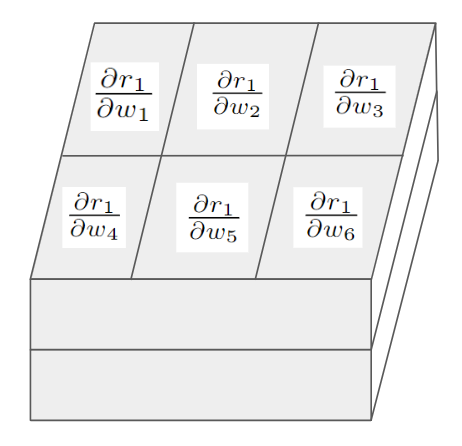
\includegraphics[width=5cm, scale=1]{images/3d_tensor.PNG}
        \captionsetup{justification=centering}
        \caption{Rank-3 tensor}
    \end{figure}

\end{subequations}


\subsection{Derivative of Matrix wrt Matrix}
\begin{subequations}
    \begin{equation}
        \text{We have matrix } \boldsymbol{A} = \begin{bmatrix}
                                                    a_{1} & a_{2}\\
                                                    a_{3} & a_{4}
                                                  \end{bmatrix},
        \text{matrix } \boldsymbol{W} = \begin{bmatrix}
                                            w_{1} & w_{2} & w_{3}\\
                                            w_{4} & w_{5} & w_{6}
                                        \end{bmatrix}
    \end{equation}
    \begin{equation}
        \renewcommand*{\arraystretch}{1.5}
        \text{We have that } \frac{\partial \boldsymbol{A}}{\partial \boldsymbol{W}} = \begin{bmatrix}
                                                                                            \frac{\partial a_{1}}{\partial \boldsymbol{W}} & \frac{\partial a_{2}}{\partial \boldsymbol{W}}\\
                                                                                            \frac{\partial a_{3}}{\partial \boldsymbol{W}} & \frac{\partial a_{4}}{\partial \boldsymbol{W}}
                                                                                        \end{bmatrix}
        \text{ , where each } \frac{\partial a_{i}}{\partial \boldsymbol{A}} \text{ is a Scalar-Matrix derivative}
    \end{equation}
    \begin{equation}
        \text{Notice that if } \boldsymbol{A} \in \mathds{R}^{m*n} \text{ and } \boldsymbol{W} \in \mathds{R}^{k*l} \text{ ; then } \frac{\partial a_{i}}{\boldsymbol{W}} \in \mathds{R}^{k*l} \text{ , } \frac{\partial \boldsymbol{A}}{\partial \boldsymbol{W}} \in \mathds{R}^{(k*l*m)*(n)}
    \end{equation}
\end{subequations}

\newpage
\subsection{Derivative of Vector wrt Matrix - Alternative methods}
Suppose that $\boldsymbol{W} \in \mathds{R}^{n*m}$ and $\boldsymbol{x} \in \mathds{R}^{m*1}$. How do we calculate $\frac{d \boldsymbol{W}\boldsymbol{x}}{d \boldsymbol{W}}$?

We know that the quantity in question is a $3^{rd}$ order tensor.

\subsubsection{Index Notation}
\begin{subequations}
    \begin{equation}
        \text{We know that } \boldsymbol{f} = \boldsymbol{W}\boldsymbol{x}
    \end{equation}
    \begin{equation}
        \text{Define } \boldsymbol{f}_{i} = \boldsymbol{W}_{ij}\boldsymbol{x}^{j} \text{ ; Note that we are using Einstein summation notation}
    \end{equation}
    \begin{equation}
        \frac{\partial \boldsymbol{f}_{i}}{\partial \boldsymbol{W}_{mn}} =
        \frac{\partial \boldsymbol{f}_{i}}{\partial \boldsymbol{W}_{ij}} \frac{\partial \boldsymbol{W}_{ij}}{\partial \boldsymbol{W}_{mn}} = 
        \frac{\partial \boldsymbol{f}_{i}}{\partial \boldsymbol{W}_{ij}} \boldsymbol{x}_{j} =
        \delta_{im}\delta_{jn}\boldsymbol{x}_{j} = \delta_{im}\boldsymbol{x}_{n}
    \end{equation}
\end{subequations}

\subsubsection{Vectorization}
\begin{equation}
    \begin{aligned}[t]
        \boldsymbol{f} &= \boldsymbol{W}\boldsymbol{x}\\
                       &= \boldsymbol{I}\boldsymbol{W}\boldsymbol{x}\\
                       &= (\boldsymbol{x}^{T} \ \otimes \boldsymbol{I}) \ vec(\boldsymbol{W})\\
                       &= (\boldsymbol{x}^{T} \ \otimes \boldsymbol{I}) \ \boldsymbol{w}
    \end{aligned}
\end{equation}
\begin{equation}
    \text{Thus, } \frac{\partial \boldsymbol{f}}{\partial \boldsymbol{w}} = (\boldsymbol{x}^{T} \otimes \boldsymbol{I})
\end{equation}

\subsubsection{Special Case}
See matrixDifferentiation.pdf for more

\newpage
\section{2-layer NN}

\subsection{Backpropagation - Bias terms}
Note that we are considering backpropagation w.r.t a single \textbf{layer}, where a single layer may encapsulate \textbf{more than one neuron}

\begin{subequations}
    \begin{equation}
        \text{Input data } \boldsymbol{X} = \begin{bmatrix}
                                                x_{11} & x_{12} & x_{13} & x_{14}\\
                                                x_{21} & x_{22} & x_{23} & x_{24}
                                            \end{bmatrix} \in \mathds{R}^{N*D}
        \text{ ; $N = $ numSamples, $D = $ dataDimension}
    \end{equation}
    \begin{equation}
        \text{Weights } \boldsymbol{W} = \begin{bmatrix}
                                            w_{11} & w_{12} & w_{13}\\
                                            w_{21} & w_{22} & w_{23}\\
                                            w_{31} & w_{32} & w_{33}\\
                                            w_{41} & w_{42} & w_{43}
                                         \end{bmatrix} \in \mathds{R}^{D*C}
        \text{ ; $C = $ number of classes}
    \end{equation}
    \begin{equation}
            \text{Bias vector } \boldsymbol{b} = \begin{bmatrix}
                                                    b_{1} & b_{2} & b_{3}
                                                 \end{bmatrix} \in \mathds{R}^{C}
    \end{equation}
    \begin{equation}
            \text{Bias matrix } \boldsymbol{B} = \begin{bmatrix}
                                                    b_{1} & b_{2} & b_{3}\\
                                                    b_{1} & b_{2} & b_{3}
                                                \end{bmatrix} \in \mathds{R}^{N*C}
            \text{; Bias vector is 'broadcast' once for each data sample}
    \end{equation}
    \begin{equation}
        \begin{aligned}[t]
            \text{Upstream term } \boldsymbol{Z} &= \boldsymbol{X}\boldsymbol{W} + \boldsymbol{B}\\
                                                 &= \begin{bmatrix}
                                                        xw_{11} & xw_{12} & xw_{13}\\
                                                        xw_{21} & xw_{22} & xw_{23}
                                                    \end{bmatrix} +
                                                    \begin{bmatrix}
                                                        b_{1} & b_{2} & b_{3}\\
                                                        b_{1} & b_{2} & b_{3}
                                                    \end{bmatrix}\\
                                                 &= \begin{bmatrix}
                                                        z_{11}  & z_{12} & z_{13}\\
                                                        z_{21}  & z_{22} & z_{23}
                                                    \end{bmatrix}
                                                    \in \mathds{R}^{N*C}
        \end{aligned}
    \end{equation}
\end{subequations}
\begin{subequations}
    \begin{equation}
        \renewcommand*{\arraystretch}{1.5}
        \begin{aligned}[t]
            \frac{\partial L_{i}}{\partial \boldsymbol{b}} &= \frac{\partial L_{i}}{\partial \boldsymbol{Z}_{i}} \cdot \frac{\partial \boldsymbol{Z}_{i}}{\partial \boldsymbol{b}} \text{ ; $\boldsymbol{Z}_{i}$ stands for $i^{th}$ row of $\boldsymbol{Z}$ (corresponding to $i^{th}$ sample), $L_{i}$ stands for loss of $i^{th}$ sample}\\
                                                           &= \frac{\partial L_{i}}{\partial \boldsymbol{Z}_{i}} \cdot \frac{\partial}{\partial \boldsymbol{b}}
                                                                   \begin{bmatrix}
                                                                       z_{i1} & z_{i2} & z_{i3}
                                                                   \end{bmatrix}\\
                                                           &= \frac{\partial L_{i}}{\partial \boldsymbol{Z}_{i}} \cdot 
                                                                   \begin{bmatrix}
                                                                       \frac{\partial z_{i1}}{\partial b_{1}} & \frac{\partial z_{i1}}{\partial b_{2}} & \frac{\partial z_{i1}}{\partial b_{3}}\\
                                                                       \frac{\partial z_{i2}}{\partial b_{1}} & \frac{\partial z_{i2}}{\partial b_{2}} & \frac{\partial z_{i2}}{\partial b_{3}}\\
                                                                       \frac{\partial z_{i3}}{\partial b_{1}} & \frac{\partial z_{i3}}{\partial b_{2}} & \frac{\partial z_{i3}}{\partial b_{3}}\\
                                                                   \end{bmatrix}
                                                               = \frac{\partial L_{i}}{\partial \boldsymbol{Z}_{i}} \cdot 
                                                                   \begin{bmatrix}
                                                                       1 & 0 & 0\\
                                                                       0 & 1 & 0\\
                                                                       0 & 0 & 1
                                                                   \end{bmatrix}\\
                                                           &= \frac{\partial L_{i}}{\partial \boldsymbol{Z}_{i}} \in \mathds{R}^{1*C}
        \end{aligned}
    \end{equation}
    \begin{equation}
        \text{Thus, } \frac{\partial L}{\partial \boldsymbol{b}} = \sum\limits_{i}\frac{\partial L_{i}}{\partial \boldsymbol{b}}
                                                                 = \sum\limits_{i}\frac{\partial L_{i}}{\partial z_{i}}
    \end{equation}
\end{subequations}
\end{document}